\subsection{Эллипс}
\begin{minipage}{0.5\tw}
{\bfseries \term{Эллипс}} --- плоская замкнутая кривая, сумма расстояний от любой точки которой до двух фиксированных точек, называемых фокусами, постоянна и равна удвоенной большой полуоси эллипса.
\begin{equation}
|F_1 M|+|F_2M|=\const=2a
\end{equation}	
Главные отрезки эллипса: \term{большая полуось} ($a$), \term{малая полуось} ($b$), \term{фокальное расстояние} ($c$). Очевидно,
\end{minipage}
\begin{minipage}{0.5\tw}
	\begin{flushright}
		\vspace{-.5pc}
		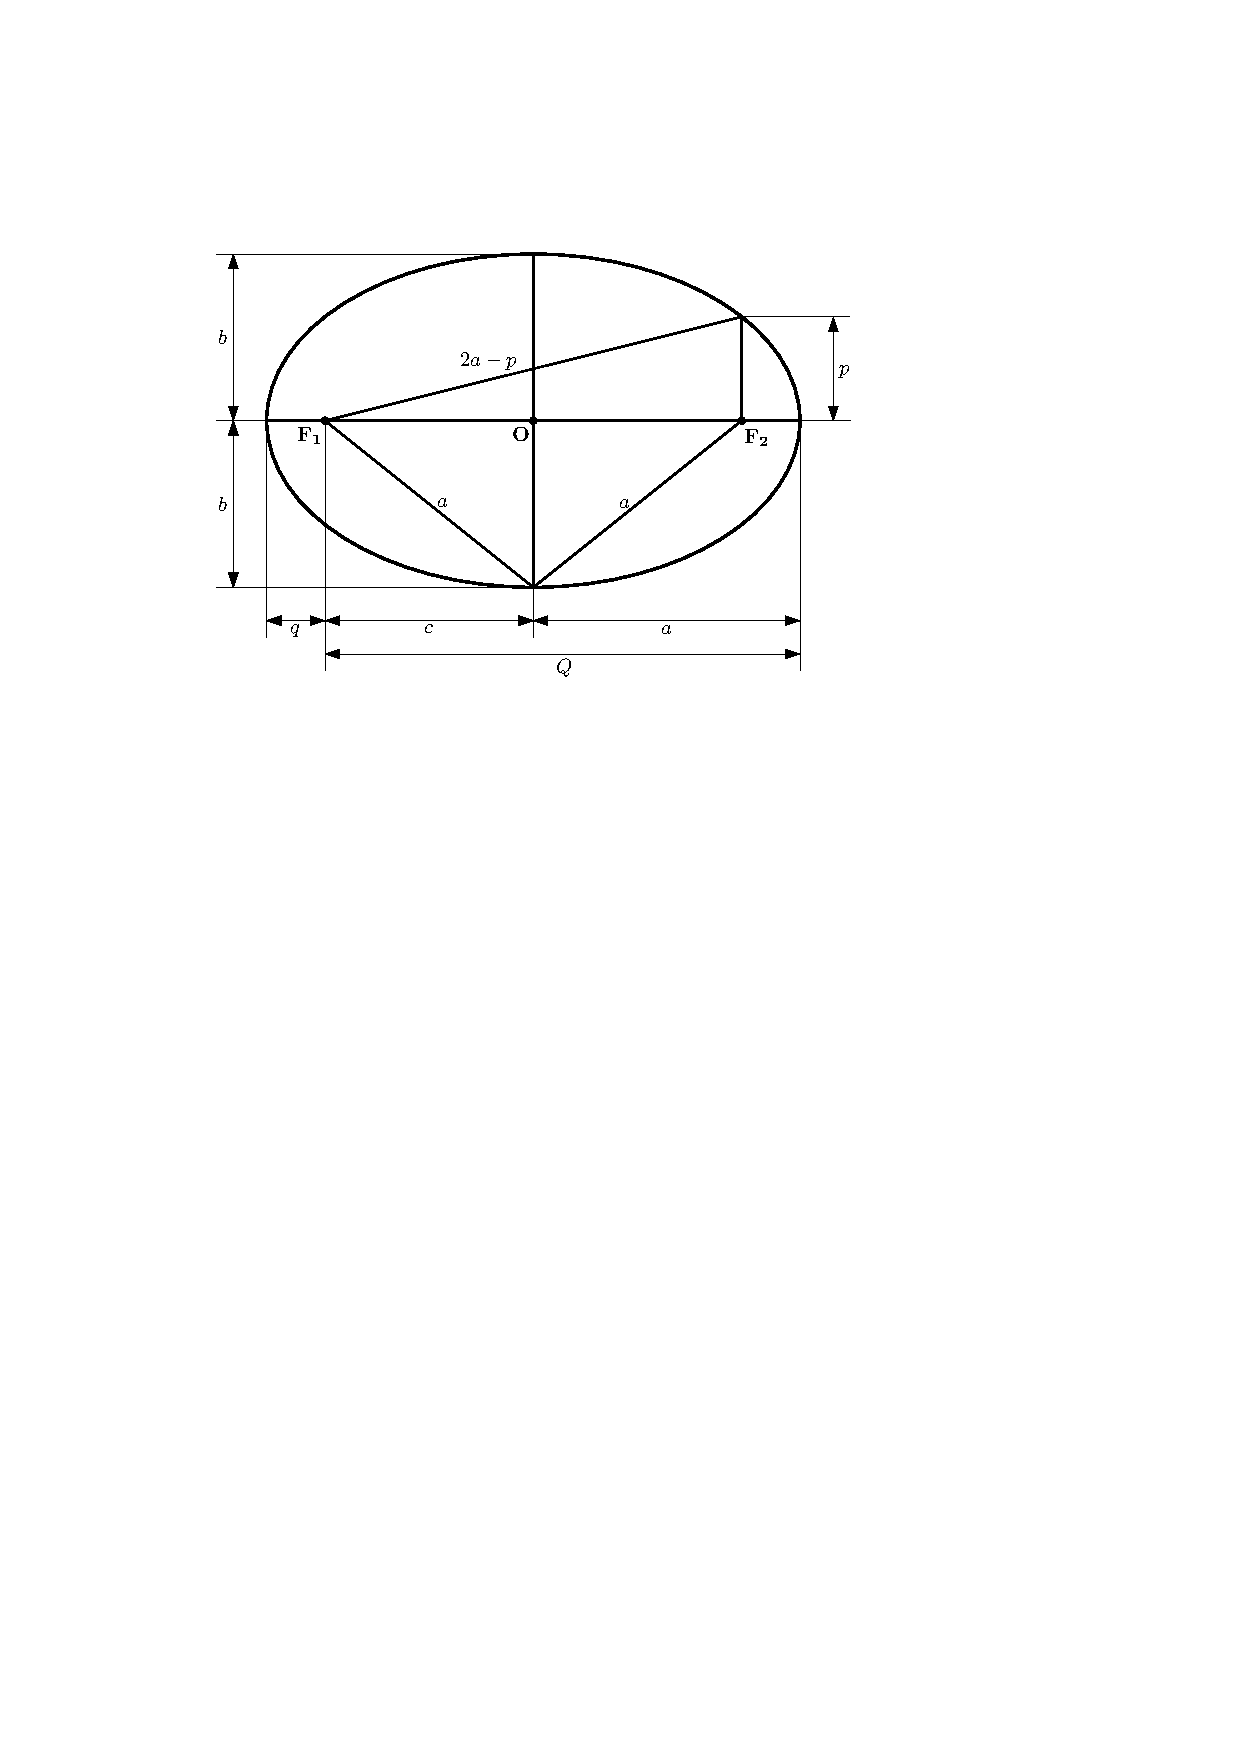
\includegraphics[width = .97\tw]{Ellips}
		\captionof{figure}{Эллипс}
	\end{flushright}
\end{minipage}\\
\begin{equation}
	b^2 + c^2 = a^2.
\end{equation}
\term{Эксцентриситет} ($e$)~--- числовая 
характеристика, показывающая степень отклонения от 
окружности. Для эллипса $e$ лежит в интервале $(0, \, 1)$ и
определяется формулой\begin{equation}
	e = \frac{c}{a}.
\end{equation}

\term{Апоцентр}~--- наиболее удаленная точка
от заданного фокуса точка эллипса. Из определения эллипса
вытекает соотношение для расстояния от фокуса до 
апоцентра ($Q$):\begin{equation}
Q = a (1 + e).
\end{equation}

\term{Перицентр}~--- ближайшая точка
точка эллипса к заданному фокусу. Из определения эллипса
вытекает соотношение для расстояния от фокуса до 
перицетра ($q$):\begin{equation}
q = a (1 - e).
\end{equation}

\term{Фокальный параметр}~($p$)~--- длина перпендикуляра,
проведенного из фокуса до точки пересечения с эллипсом.
Из теоремы Пифагора и определения эллипса следует 
нижеприведенная формула для расчета его длины:
\begin{equation}
p=\frac{b^2}{a}=a(1-e^2)=b\sqrt{1-e^2}.
\end{equation}

\term{Площадь эллипса} ($S$) --- площадь части 
плоскости, ограниченной эллипсом, равна
\begin{equation}
S=\pi ab = \pi a^2 \sqrt{1-e^2}.
\end{equation}

%Радиус кривизны дуги эллипса в зависимости от расстояния 
%$x$ от фокуса:
%\begin{equation}
%R=\frac{(2ax-x^2)^{3/2}}{ab}
%\end{equation}
%\begin{center}
%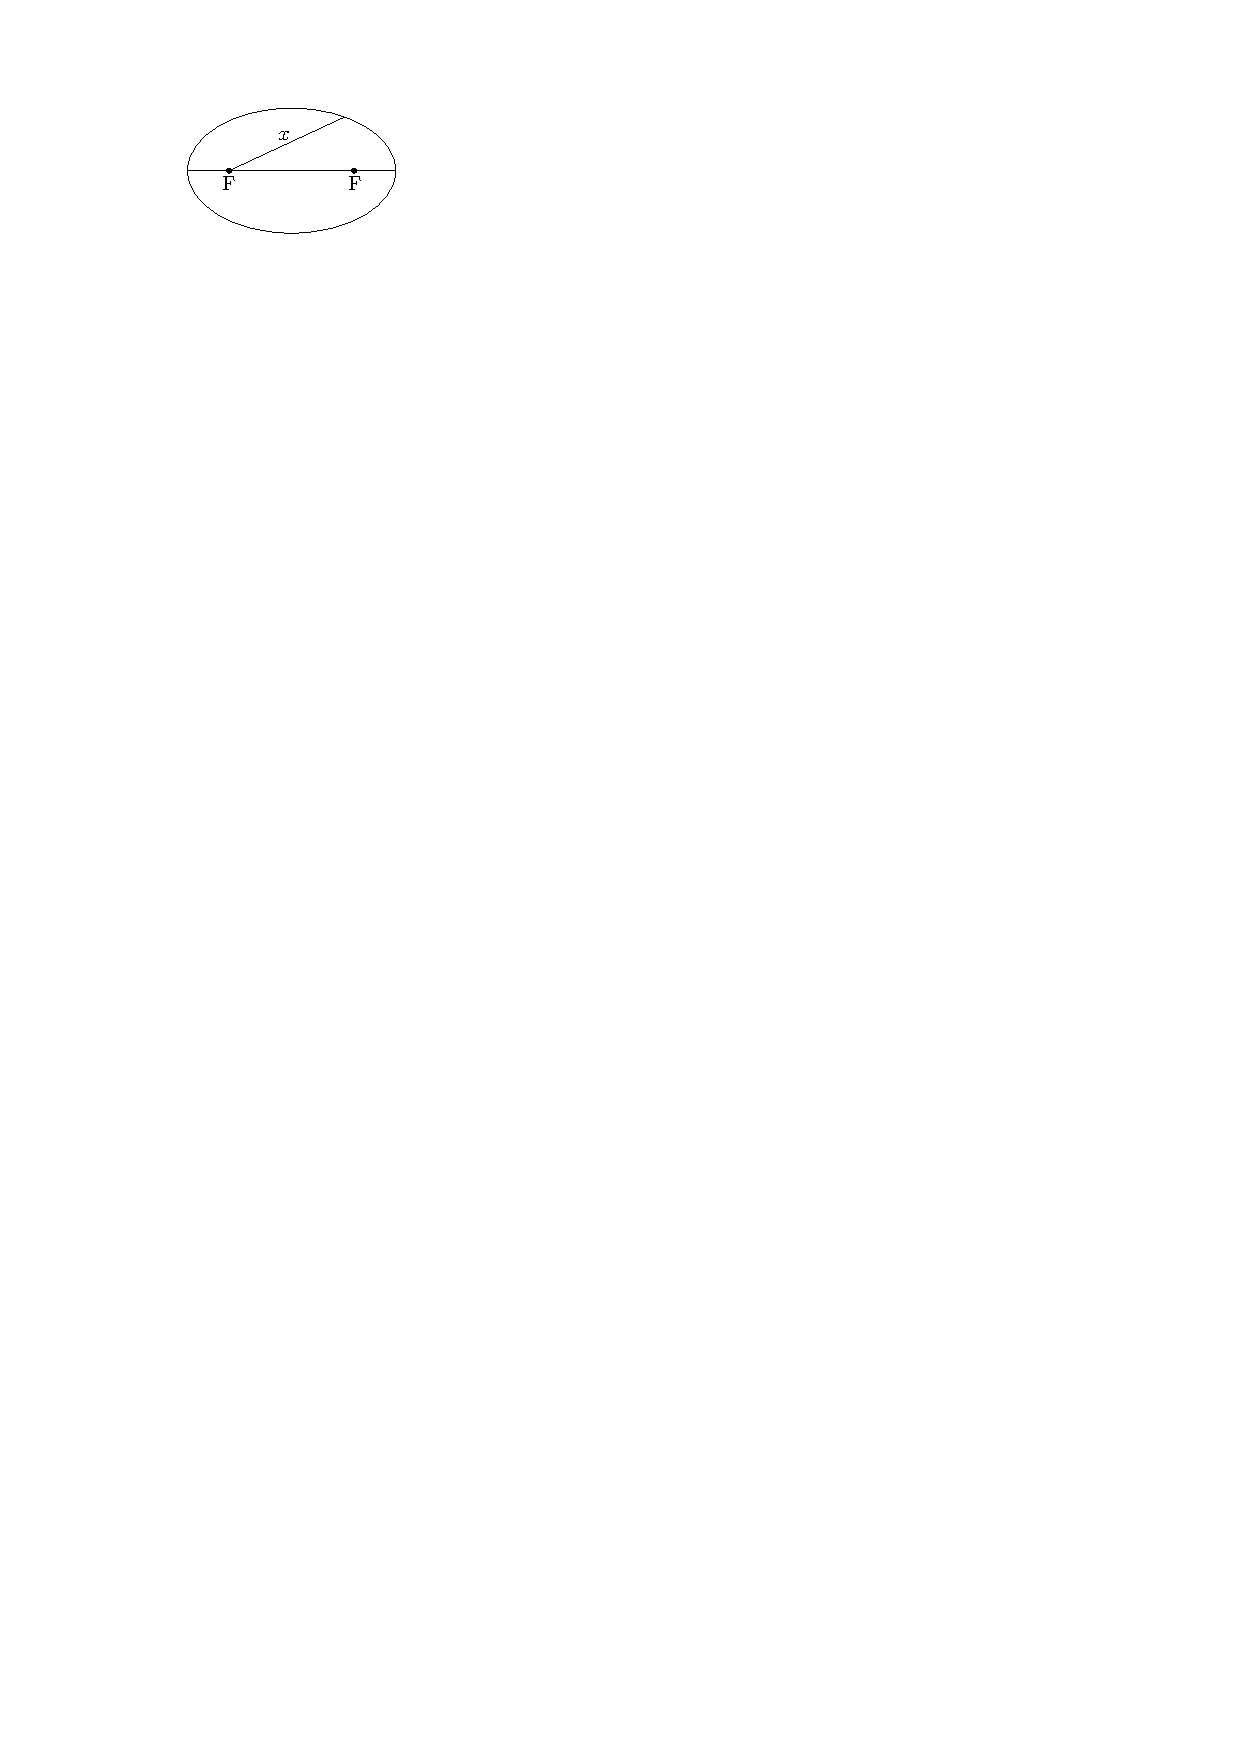
\includegraphics[width = 0.3\textwidth]{rad-curv}
%\begin{figure}[!h]
%\caption{К вычислению радиуса кривизны эллипса}
%\end{figure}
%\end{center}

{\itshape Уравнение эллипса} в декартовых координатах 
представляет собой уравнение замкнутой кривой второго 
порядка, канонический вид которого:
\begin{equation}
\frac{x^2}{a^2}+\frac{y^2}{b^2}=1.
\end{equation}

Его можно представить параметрическом виде:\begin{equation}
\left\{\begin{aligned}[lcl]
&x=a\cos t,\\
&y=b\sin t;\\
\end{aligned}
\right. \quad\quad t \in [0, \, 2\pi).
\end{equation}
В полярных координатах уравнение принимает следующий вид:
\begin{equation}
r=\frac{p}{1\pm e \cos \varphi},
\label{eq:ellipse-pol-eq}
\end{equation} 
\begin{wrapfigure}[11]{l}{0.5\tw}
	\centering
	\vspace{-.7pc}
	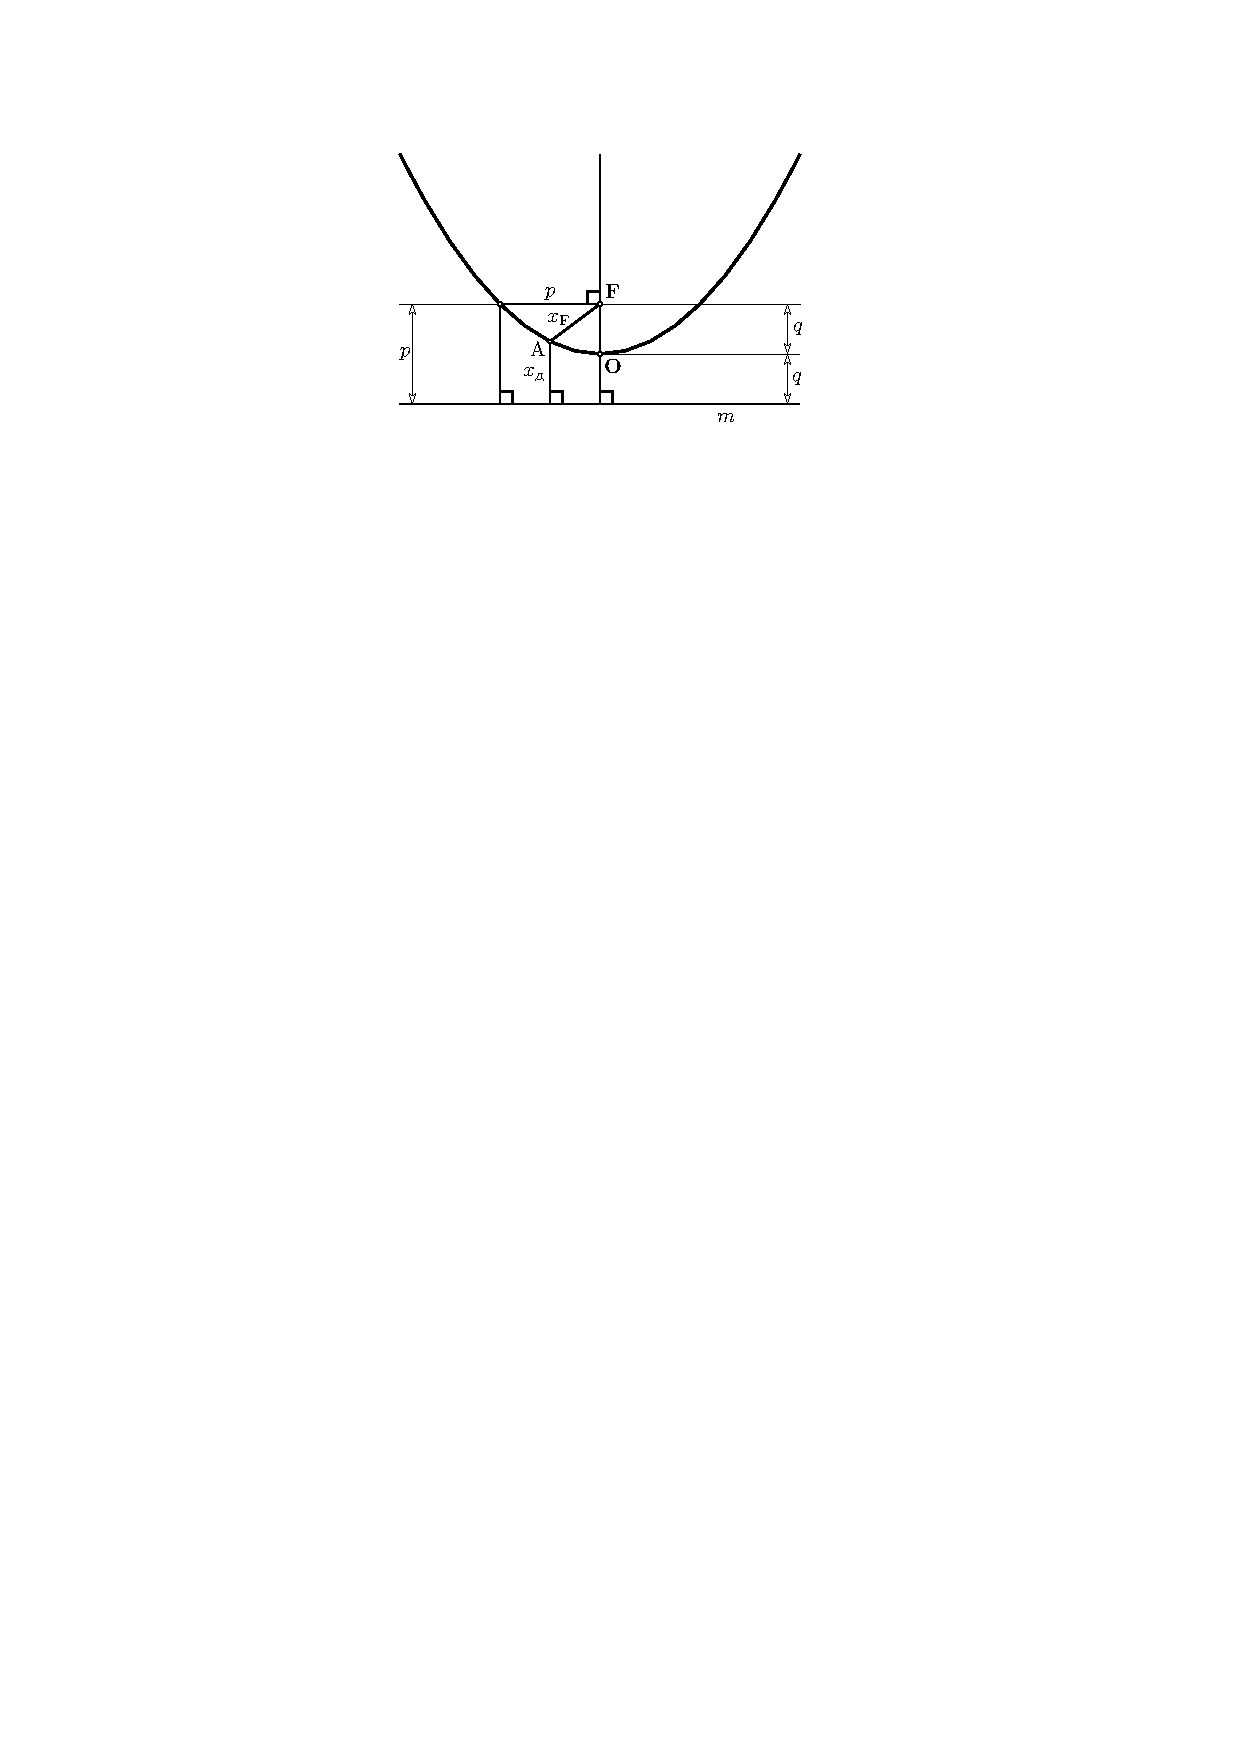
\includegraphics[width = 0.5\tw]{Parabola}
	\captionof{figure}{Парабола \label{pic:the-pic}}
\end{wrapfigure}
где $\varphi$ --- \term{истинная аномалия} --- угол 
{\slshape перицентр -- фокус -- заданная точка}, 
отсчитываемый в сторону движения по эллипсу. При 
знаке плюс перед $e$ второй фокус эллипса будет 
находится в точке $(0, \, 2c)$, а при минус --- в 
точке $(\pi, \, 2c)$.

Кроме этого, эллипс обладает важным {\itshape оптическим 
свойством}, которое можно сформулировать так: свет от источника в одном из фокусов, 
	отражается эллипсом так, что отражённые лучи пересекаются 
	во втором фокусе или, что тоже самое, касательная к эллипсу в заданной точке образует с фокальными радиусами в данной точке равные острые углы.






 
